\begin{figure*}[t]
\centering
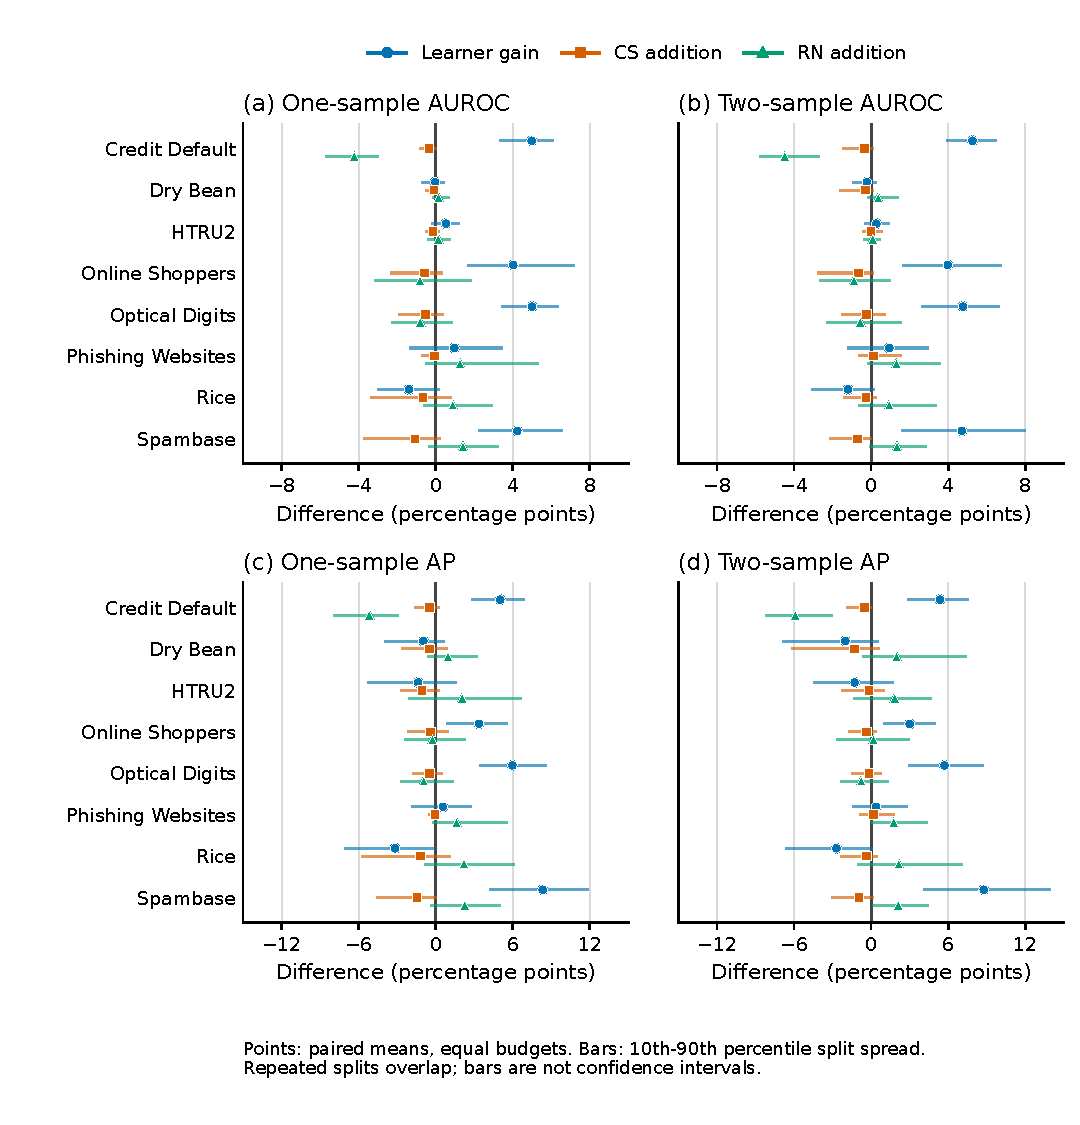
\includegraphics[width=\textwidth]{main/figures/fig_real_decomposition.pdf}
\caption{Real-data learner-versus-strategy decomposition. Learner gain is naive CatBoost minus logistic probability correction; CS and RN additions compare the respective PU strategy with naive CatBoost. Each dataset point averages 20 paired repeated splits within each label budget and then the two budgets equally. Bars show the empirical 10th--90th percentile of the 40 paired split contrasts, a descriptive balanced-budget mixture. Repeated splits are not independent datasets; these bars are not confidence intervals. Dataset order is fixed, and no winner or group maximum is selected.}
\label{fig:real-decomposition}
\end{figure*}
